\documentclass{beamer}

\usepackage[utf8]{inputenc}
\usepackage[frenchb]{babel}
\usepackage{lmodern}
\usepackage{amsmath}
\usepackage{graphicx}
\usepackage{amssymb}
\usepackage{numprint}
\usepackage{tikz}
\usepackage{pgfplots}
\usepackage{mathrsfs}
\usetheme{Warsaw}

\title{APP3: Le rayonnement électromagnétique}
\author{Groupe 1254}
%\author{\bsc{Paulus} L.,\bsc{Joachim} C. , \bsc{Goyens} V., \bsc{Boigelot} S., \bsc{Xavier} L., \bsc{Sliti} A., \bsc{Nicol} E.}

\begin{document}
\begin{frame}
	\maketitle
\end{frame}
\begin{frame}{Question 1}
	\begin{columns}
		\begin{column}{0.40\textwidth}
			\begin{center}
	    		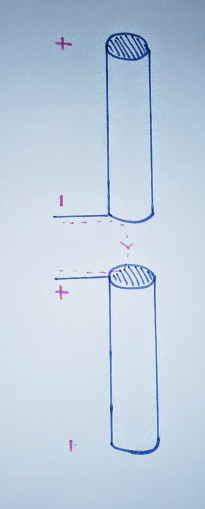
\includegraphics[scale=0.3, angle=90]{question1.png}
        		\end{center}
        	\end{column}
        	\begin{column}{0.40\textwidth}
			\begin{center}
	    Je sais pas trop quoi dire ...
        	\end{center}
        	\end{column}
        	\end{columns}
        	
        	\end{frame}
\begin{frame}{Question 1}
	\begin{columns}
		\begin{column}{0.40\textwidth}
			\begin{center}
	    		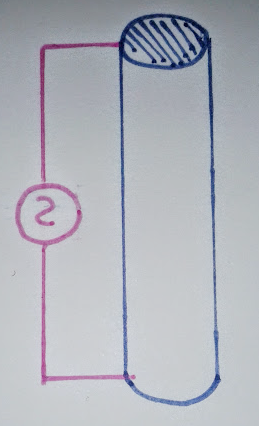
\includegraphics[scale=0.2, angle=90]{Question1-2.png}
        		\end{center}
        	\end{column}
        	\begin{column}{0.40\textwidth}
			\begin{center}
	    Je sais pas trop quoi dire ...
        	\end{center}
        	\end{column}
        	\end{columns}
\end{frame}
\begin{frame}{Question 2}
	\begin{columns}
		\begin{column}{0.40\textwidth}
			\begin{center}
	    		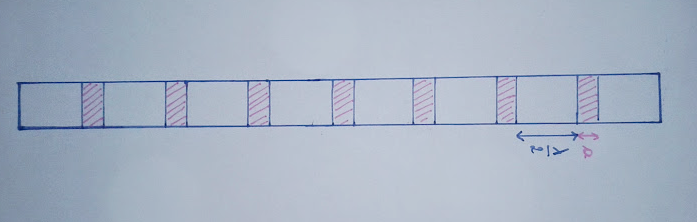
\includegraphics[scale=0.25, angle=90]{Question2.png}
        		\end{center}
        	\end{column}
        	\begin{column}{0.40\textwidth}
			\begin{center}
	    \begin{enumerate}
	    \item 1 antenne:$$ \left( \frac{\sin x}{x}\right)^2$$
	    \item $n$ antennes: $$ \left( \frac{\sin nx}{\sin x}\right)^2 \cdot \left( \frac{\sin x}{x}\right)$$
	    \end{enumerate}
        	\end{center}
        	\end{column}
        	\end{columns}
\end{frame}
\end{document}